\documentclass[12pt,a4paper,oneside]{book}
\usepackage[italian]{babel}
\usepackage[UTF8]{inputenc}
%\usepackage[latin1]{inputenc}
\usepackage{amsmath}
\usepackage{amsfonts}
\usepackage{amssymb}
\usepackage{graphicx}
\usepackage{eso-pic}
\usepackage{setspace}
\usepackage{fancyhdr} 
\newcommand{\fncyblank}{\fancyhf{}}
\newenvironment{abstract}% 
{\cleardoublepage\fncyblank\null \vfill\begin{center}% 
\bfseries \abstractname \end{center}}% 
{\vfill\null}
\newcommand\AlCentroPagina[1]{% 
\AddToShipoutPicture*{\AtPageCenter{%
\makebox(0,0){\includegraphics%
[width=1\paperwidth]{#1}}}}}
\setlength{\parindent}{0pt}
\setlength{\parskip}{1ex plus 0.5ex minus 0.2ex}
\author{Maria Luisa Feola}
\title{Reti Neurali}

%`` e '': sono le virgolette del TeX; non esistono, nel TeX, le virgolette semplici ( " ) come in Word; le virgolette `` nella tastiera italiana vengono ottenute con la combinazione di tasti “ALT + 96”, mentre le altre sono il segno dell'apostrofo;

% ~ ALT+126 tilde da mettere tra due parole per non farle staccare quando si va a capo

\begin{document}
%FRONTESPIZIO
	\AlCentroPagina{IMMAGINI/Frontespizio}\thispagestyle{empty}
	
%DEDICA
	\begin{flushright} 
		\newpage
		\null\vspace{\stretch{1}}
		\thispagestyle{empty}
		\textit{Grazie PAINT}
		\vspace{\stretch{2}}\null
	\end{flushright} 
%FINE DEDICA
   	
%FRASE
   	\begin{flushright} 
   		\newpage
   		\null\vspace{\stretch{1}}
   		\thispagestyle{empty}
   		\textit{Se non puoi passare attraverso una montagna, giraci intorno; \\ se non puoi girarci intorno, passaci sopra;\\ se non puoi passarci sopra, siediti un attimo \\e chiediti se raggiungere l'altro lato sia davvero così importante.\\ \vspace{1cm} Se lo è comincia a scavare una galleria.}
   		\vspace{\stretch{2}}\null
   	\end{flushright} 
%FINEFRASE
   
%INDICE
	\tableofcontents\thispagestyle{empty}
%FINE INDICE
	
%INTRODUZIONE
	\chapter*{Introduzione}
	\onehalfspacing
	\addcontentsline{toc}{chapter}{Introduzione}
	prova
%FINE INTRODUZIONE
		
%INIZIO DEL PRIMO CAPITOLO
	
	\chapter{ Presentazione delle reti neurali }
	
	
	
	\section{Cenni storici ed origini}
		Le reti neurali artificiali, dall'inglese \textit{Artificial Neural Network (ANN)}, e la conseguente computazione neurale, sono state costruite ispirandosi ai sistemi neurali biologici, con l'obiettivo di modellarne il comportamento e la struttura e di simularne le funzioni basilari e fondamentali.\\
		Una definizione semplice e formale di tali strutture è fornita dall'inventore del primo neurocomputer, il Dr. Robert Hecht-Nielsen che le definì come: \\
		
		\textit{«...a computing system made up of a number of simple, highly interconnected processing elements, which process information by their dynamic state response to external inputs»}\\
		\textit{(da Neural Network Primer: Parte uno, Maureen Caudill, 1989)}\\
		
		Tradotto in italiano \\
		\textit{«... un sistema di calcolo costituito da una serie di semplici, altamente interconnessi elementi di elaborazione, che elaborano le informazioni attraverso il loro stato dinamico rispondendo agli input esterni.»}\\
		
		Le basi per lo studio di tali reti furono poste dallo psichiatra Warren McCulloch e del matematico Walter Pitts, i quali riuscirono a riprodurre una rete neurale utilizzando semplici circuiti elettrici collegati tra loro. Questa collaborazione portò alla luce l'analogia che sussiste tra le reti neurali e la macchina di Turing ed in tal modo si capì che qualsiasi operazione eseguita da una rete neurale poteva essere eseguita anche da un computer; infatti le reti che furono prodotte risultavano essere automi a stati finiti in grado di realizzare la logica delle proposizioni e di formulare ipotesi sulla natura dei meccanismi cerebrali, il tutto equivalentemente ad un programma per computer. Il frutto di tale lavoro fu reso noto nel 1943 con la pubblicazione del libro ``\emph{A logical calculus of the ideas immanent in nervous activity}'', nel quale fu schematizzato un combinatore lineare a soglia con dati binari multipli in entrata e un singolo dato binario in uscita.\\
	    Ciò che quindi McCulloch e Pitts riuscirono a fare è presentare un modello di neurone formale dimostrando che reti formate da tali neuroni riuscivano a computare funzioni della logica del primo ordine.\\
	    Un punto di svolta per lo studio delle reti neurali si ebbe successivamente alla pubblicazione del lavoro dello psicologo Donald Hebb, ``\emph{The Organization of Behavior}'' nel 1949. Hebb trovò una correlazione tra la psicologia del comportamento umano e la fisiologia del sistema nervoso, donando un grande contributo alla teoria sull'apprendimento associativo, teoria che risultò essere alla base dei metodi di apprendimento delle reti neurali, e che si basava sulla nota legge di Hebb: \textit{«Se un neurone A è abbastanza vicino ad un neurone B da contribuire ripetutamente e in maniera duratura alla sua eccitazione, allora ha luogo in entrambi i neuroni un processo di crescita o di cambiamento metabolico tale per cui l'efficacia di A nell'eccitare B viene accresciuta»}.\\
	    Il decennio che va dagli anni cinquanta agli anni sessanta fu totalmente influenzato dalla legge di Hebb a tal punto che numerosi gruppi di ricerca condussero esperimenti e test sulle funzionalità del cervello, fino a porre le basi per la nascita dell'intelligenza artificiale (AI).\\
	    Nel 1958 Frank Rosenblatt introdusse il primo schema di rete neurale che designò con il termine ``\textbf{\emph{perceptron}}'', in italiano percettrone, allo scopo di fornire un'interpretazione dell'organizzazione generale dei sistemi biologici attraverso un modello mirato all'analisi, in forma matematica, di funzioni quali ad esempio l'immagazzinamento delle informazioni. Il percettrone fu il primo modello di apprendimento supervisionato e presupponeva uno strato di ingresso ed uno di uscita, discriminando gli ingressi in due insiemi linearmente separabili e basandosi su una regola di apprendimento che si appellava alla minimizzazione dell'errore.\\
	    Il percettrone ancora oggi viene utilizzato in varie applicazioni e risultò essere un modello più efficace rispetto a quello binario di McCulloch e Pitts, poichè i suoi pesi sinaptici sono variabili e quindi in grado di apprendere.\\
		Nonostante, però, l'iniziale successo di tale modello e l'interesse mostrato dalla comunità scientifica, tale rete neurale non risultò abbastanza potente; le reti a due strati basate sui percettroni avevano limiti operativi, infatti non riuscivano a risolvere tutte le classi di problemi, in particolare quelli non caratterizzati dalla separabilità lineare delle soluzioni come ad esempio l'operatore \emph{XOR}, ovvero la funzione \emph{OR} esclusivo, che discrimina gli ingressi in modo non linearmente separabile.\\
		Solo negli anni ottanta, con il matematico Paul Werbos, si superarono i limiti del percettrone di Rosenblatt.  Quest'ultimo introdusse uno o più livelli intermedi all'interno delle reti neurali creando una classe chiamata  ``\textbf{\emph{Multi-Layers Perceptron}}'', ovvero percettrone multistrato, il cui metodo di addestramento principale era l'\emph{error backpropagation}, ovvero l'algoritmo di retropropagazione dell'errore, che permetteva la modifica sistematica dei pesi delle connessioni, in modo da rendere la risposta della rete quanto più vicina a quella desiderata.\\
		Tale algoritmo, proposto nel 1986 da David E.Rumelhart, G. Hinton e R. J. Williams consentì di superare le problematiche legate al percettrone di Rosenblatt e permise di risolvere il problema della separabilità non lineare delle soluzioni, rendendo quindi possibile calcolare la funzione XOR e segnando il definitivo rilancio delle reti neurali.
		
		
		
		
	\section{Analogie con il sistema nervoso ed applicazioni delle ANN}
	
		Come accennato nel paragrafo precedente, una rete neurale è un sistema computazionale costruito basandosi sui processi biologici naturali, il cui obiettivo è la riproduzione delle attività tipiche del cervello umano, ad esempio la comprensione del linguaggio, la percezione di immagini, il riconoscimento di forme  \\
		In altre parole, lo scopo di una rete neurale artificiale è l’emulazione del sistema nervoso animale, in particolar modo di quello umano, il quale presenta numerose caratteristiche che risultano essere ottime per la riproduzione di un sistema computazionale che lo imiti: è flessibile poiché si adatta ad ogni tipologia di situazione imparando, è robusto in quanto le cellule nervose muoiono ogni giorno senza avere effetti significativi sulla performance del sistema, è resistente, piccolo e dissipa poca energia. \\
		Tale riproduzione non deve essere intesa come atta alla costruzione di un cervello artificiale. Infatti le caratteristiche delle reti neurali biologiche, riprese dalla computazione neurale artificiale, sono in esigua minoranza: gli stessi neuroni artificiali sono solo un’approssimazione dei neuroni biologici e sono in grado di riprodurre solo tre dei circa centocinquanta processi che sono tipici dei neuroni del cervello umano.\\
		Il sistema nervoso umano può essere pensato, quindi, come una grande struttura computazionale formata da milioni di unità fortemente interconnesse tra loro in modo parallelo e che riesce a trasformare continui input in output ragionevoli. Le reti neurali rappresentano una riproduzione significativa di tale struttura, in particolar modo degli algoritmi di apprendimento e di ottimizzazione, basati su un modello \emph{connessionistico} di calcolo: le operazioni responsabili dello scambio di informazioni avvengono per mezzo dell'interazione tra le unità elementari. Sono sistemi altamente paralleli: fornendo i dati del problema alle unità di input, la computazione si propaga in parallelo nella rete fino alle unità di output che producono il risultato. \\
	
		\begin{figure}[h]
			\centering
			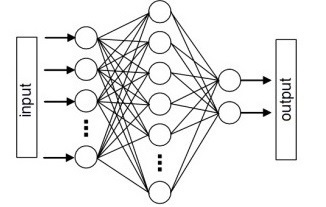
\includegraphics[width=0.6\linewidth]{IMMAGINI/esempioiniziale}
			\caption{Esempio di rete neurale}
			\label{fig:esempio}
		\end{figure}
		
		II campo tipico di applicazione delle reti neurali è quello dell'individuazione di legami di \textbf{ingresso-uscita} all'interno di sistemi complessi in cui i dati a disposizione sono molto 
		numerosi o contenenti poca informazione e quindi non risulta chiaro quali relazioni deterministiche esistano tra le diverse variabili che caratterizzano il problema. Si tratta di campi in cui l'analisi statistica di tutte le variabili risulta difficoltosa o dispendiosa in termini di calcolo.\\ 
		Ecco un breve elenco di applicazioni note:
		
		\begin{itemize}
			\item Elaborazione delle immagini (compressione e miglioramento di immagini in tempo reale);
			\item Elaborazione del suono (compressione e miglioramento in tempo reale della voce e della musica, aiuti audio e protesi ecc\dots);
			\item Rivelazione, verifica e identificazione di caratteri e oggetti (codici a barre, impronte digitali, firme, facce ecc\dots );  
			\item Riconoscimento della voce (elaborazione di parole dettate, identificazione di persone per via vocale, selezione telefonica ecc\dots );
			\item Applicazioni basate su ingressi di origine sensoriale (ingresso tattile, visivo, acustico, olfattivo);
			\item Archivi (musica, video, immagini ecc\dots);
			\item Sintesi e miglioramento dati (fax, grafica, cancellazione di rumore, apparecchiature televisive ad alta risoluzione ecc\dots);
			\item Robot autonomi.
		\end{itemize}

		
		
	\section{Il neurone biologico}
		
		Per convincersi a fondo sulla connessione tra le reti neurali artificiali e le reti neurali del sistema nervoso umano, e le numerose analogie che ne derivano, è bene dare una breve descrizione del secondo sistema, in modo da far emergere le principali caratteristiche ed i principali costituenti che sono utili al fine della comprensione delle reti neurali.\\
  		Il sistema nervoso è diviso in tre stadi:
		
		\begin{itemize}
			\item I \emph{recettori}, che convertono gli stimoli esterni in impulsi elettrici che vengono inviati alla rete neurale;
			\item La \emph{rete neurale}, la quale riceve gli impulsi elettrici provenienti dai recettori e li immagazzina come informazioni utili per poter prendere delle decisioni che vengono inviate, anch'esse sotto forma di impulsi elettrici, agli attuatori;
			\item Gli \emph{attuatori} responsabili della trasformazione degli impulsi in risposte per l'ambiente esterno.
		\end{itemize}
	
		\begin{figure}[h]
		\centering
		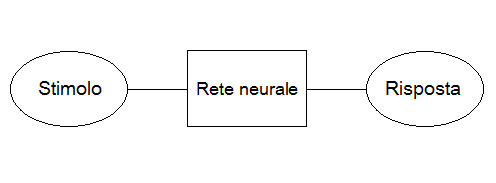
\includegraphics[width=1\linewidth]{IMMAGINI/Sistemanervoso}
		\caption{Stadi del sistema nervoso}
		\label{fig: stadi sistema nervoso}
		\end{figure}
		
		Nel sistema nervoso centrale sono presenti circa $10^{11}$ cellule nervose, i \emph{neuroni}. Tali cellule sono connesse strettamente tra loro attraverso numerosi collegamenti che nel loro insieme vanno a formare la rete neurale. \\
		Un neurone è formato da un corpo centrale, identificato con il nome di \emph{soma}, all'interno del quale è presente il nucleo, e da molti prolungamenti citoplasmatici, detti \emph{neutriti}, che si distinguono in:
		 
		 \begin{itemize}
		 	\item \emph{dendriti}, organizzati con diramazioni ad albero che costituiscono il \emph{ramo dendritico};
		 	\item \emph{assone}, la cui parte finale prende il nome di \emph{bottone sinaptico}.
		 \end{itemize}
		 
		 I dendriti ricevono segnali dai neuroni afferenti e li propagano verso il nucleo. L'assone conduce, invece, il segnale verso altre cellule grazie alla presenza del bottone sinaptico alla sua estremità, che risulta essere un'ulteriore ramificazione: quest'ultima va a formare i terminali attraverso i quali i segnali elettrici vengono trasmessi.\\
		 
		 \begin{figure}[h]
		 	\centering
		 	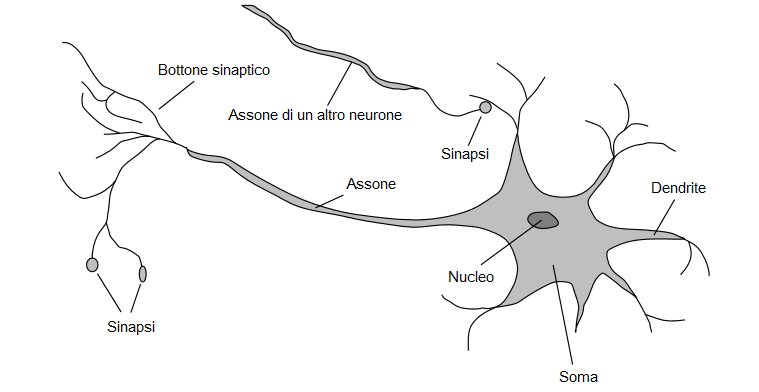
\includegraphics[width=1\linewidth]{IMMAGINI/neuron}
		 	\caption{Neurone biologico}
		 	\label{fig:neuron}
		 \end{figure}
	 
	 	\textbf{Tra un terminale di un assone e la cellula ricevente, esiste uno spazio che viene superato dagli impulsi elettrici per mezzo dei \emph{neurotrasmettitori}, sostanze chimiche che guidano le informazioni tra le cellule e che si suddividono in \emph{eccitatori} se favoriscono la creazione dell'impulso e \emph{soppressori} se inibiscono l'impulso.}\\ Il punto di connessione tra il terminale di un neurone ed il dendrite di un altro costituisce una struttura altamente specializzata che prende il nome di \emph{sinapsi} e che risulta quindi essere la responsabile delle interazioni. La sinapsi svolge due processi: un processo \emph{presinaptico} in cui viene liberato il neurotramettitore ed un processo \emph{postsinaptico}, azionato dal neurotrasmettitore, che rigenera il segnale elettrico.Quindi una sinapsi converte un segnale elettrico in chimico durante il processo postsinaptico per poi riconvertirlo in elettrico durante la postsinapsi.\\ 
	 	Un neurone trasmette un impulso elettrico lungo il suo assone nel momento in cui si verifica una differenza di potenziale elettrico tra l’interno e l’esterno della cellula, provocando la liberazione di un neurotrasmettitore di cui sopra.
		
		
		 
	\section{Modello del neurone artificiale}
		
		La breve illustrazione del sistema neurale umano nel paragrafo precedente suggerisce uno schema per delineare l'organizzazione delle reti neurali artificiali: queste ultime sono formate da un elevato numero di unità computazionali, che possono essere equiparate ai neuroni umani, capaci di eseguire una somma pesata. Tali unità sono collegate tra loro attraverso delle connessioni, così come le sinapsi collegano i neuroni nella rete umana. \\
		Consideriamo una generica unità $j$ costituita da $n$ canali di ingresso $x_{1}, x_{2}, ... ,x_{n}$.
		Gli input provenienti da strati precedenti o direttamente dall'esterno entrano nel neurone tramite tali canali.

		\begin{figure}[h!]
			\centering
			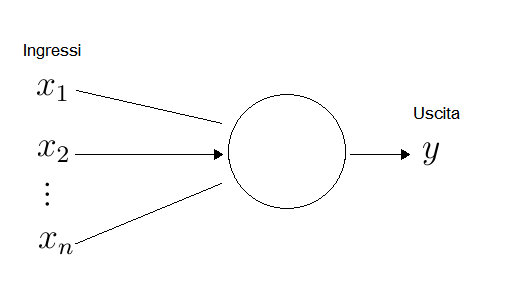
\includegraphics[width=0.7\linewidth]{IMMAGINI/palla1}
			\caption{Canali di ingresso in un neurone}
			\label{fig:palla1}
		\end{figure}
		
		Sulle connessioni sono presenti dei \emph{pesi sinaptici} $w_{i}$, numeri reali che denotano l'\emph{efficacia sinaptica}, ovvero la forza della connessione. Se $w_{i}>0$ il canale è detto \emph{eccitatorio}, se $w_{i}<0$ il canale è \emph{inibitorio}.\\
		I segnali in entrata, pesati dalle rispettive sinapsi, sono convogliati nel \emph{soma} del neurone artificiale, all'interno del quale vengono sommati producendo una combinazione lineare così definita:
		
		\begin{equation} 
			\label{eqn:net} 
				$$ \begin{center} $\sum\limits_{i=1}^n w_{i}x_{i}$ \end{center}$$
		\end{equation} 
		
		La somma pesata degli ingressi viene indicata con la parola \emph{net} ed il segnale con cui il neurone trasmette la sua attività all'esterno è calcolato applicando una \emph{funzione di attivazione} $\varphi$ che limita l'ampiezza dell'output; si assume per comodità che le ampiezze degli output appartengono all'intervallo $[0,1]$ oppure $[-1,1]$.
		
		\begin{figure}[h!]
			\centering
			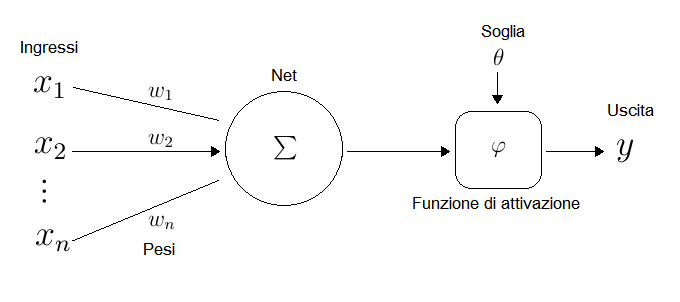
\includegraphics[width=1\linewidth]{IMMAGINI/palla2}
			\caption{Modello neurone}
			\label{fig:palla2}
		\end{figure}
		
		\clearpage
		Il modello neuronale include anche un valore \emph{soglia} che ha l'effetto, a seconda della sua positività o negatività, di aumentare o diminuire il valore in ingresso alla funzione di attivazione.\\
		L'output finale sarà allora:
		
		\begin{equation}
			\label{eqn:output1} 
				$$\begin{center} $y= \varphi (\sum\limits_{i=1}^n w_{i}x_{i})$  \end{center}$$
		\end{equation}
	
		E se indichiamo con $\theta$ il valore di soglia, la~\eqref{eqn:output1} diventerà:
		\begin{equation}
			\label{eqn:output2}
				$$\begin{center} $y= \varphi (\sum\limits_{i=1}^n w_{i}x_{i}-\theta)$  \end{center}$$
		\end{equation}
		
		Interpretando la soglia come il peso associato ad un ulteriore canale di ingresso $x_{0}$, e quindi $w_{0}=\theta$, potremmo anche scrivere : 
		
		\begin{equation}
			\label{eqn:output3}
				$$\begin{center} $y= \varphi (\sum\limits_{i=0}^n w_{i}x_{i})$ \end{center}$$
		\end{equation}
		
		\clearpage
		Il modello finale sarà:
		
		\begin{figure}[h!]
			\centering
			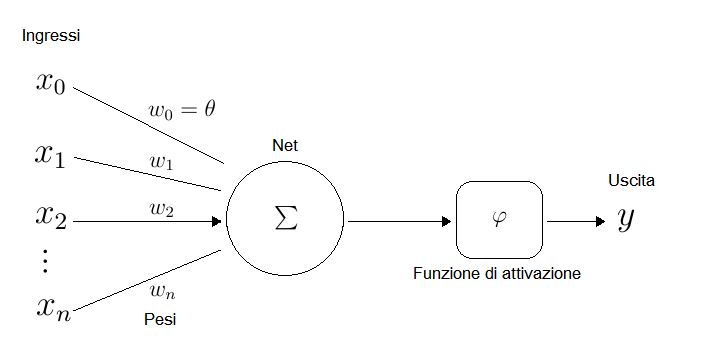
\includegraphics[width=1\linewidth]{IMMAGINI/palla3}
			\caption{ Modello neurone con soglia }
			\label{fig:palla3}
		\end{figure}
		
		L'effetto di un segnale $ x_{i} $ sul neurone è quindi uguale al prodotto 
		$w_{i}$ $\cdot$ $x_{i}$ dove $w_{i}$ è il peso attribuito alla sinapsi corrispondente ed il potenziale di attivazione è dato dalla somma algebrica dei prodotti di tutti i segnali di ingresso e dei valori dei pesi corrispondenti.\\
	 	Schematizzando, ed individuando il neurone artificiale come l'unità di calcolo fondamentale della rete neurale, gli elementi base che lo rappresentano sono:
		
		\begin{itemize}
			\item Un insieme di connessioni;
			\item Un sommatore;
			\item Una funzione di attivazione;
			\item Un valore di soglia.
		\end{itemize}
		
		
		\clearpage
	\section{Attivazione di un neurone e funzioni di attivazione}
		
		Nelle reti neurali si può avere una \emph{attivazione asincrona}, in cui i neuroni si attivano uno per volta, ed una {attivazione sincrona} in cui tutti i neuroni si attivano contemporaneamente. L'attivazione di un neurone dipende solo dall'informazione ricevuta ed è indipendente dalle operazioni svolte dagli altri nodi.\\ 
		La funzione di attivazione determina il tipo di risposta che un neurone è in grado di emettere. Definisce, quindi, l’uscita di un neurone in funzione del livello di attivazione. L'uscita può essere un numero reale, un numero reale appartenente ad un intervallo, oppure un numero appartenente ad un insieme discreto.\\
		
		\subsection{Funzione a soglia}
		
		Imponendo $a=\sum\limits_{i=0}^n w_{i}x_{i}$, il valore di uscita di un neurone assunto tramite una funzione a soglia é:
		
		\begin{equation}
		\label{eqn:sistemafunzioneasoglia} 
		$$ \begin{center} 
				$y=\varphi(a)=$
					$\begin{cases}
						1 \hspace{0.8cm}se\hspace{0.1cm} a \geq 0 \\
						0 \hspace{0.8cm}se\hspace{0.1cm} a < 0
					\end{cases}$
			\end{center} $$
		\end{equation}
		
		\clearpage
		ed il grafico relativo
		
		\begin{figure}[h!]
			\centering
			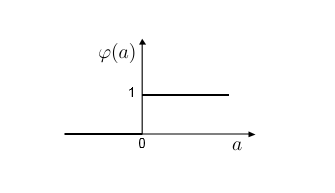
\includegraphics[width=0.6\linewidth]{IMMAGINI/asoglia}
			\caption{ Funzione di attivazione a soglia }
			\label{fig:asoglia}
		\end{figure}
	
		Se si tralascia il contributo dell'ingresso $x_{0}$ dal livello di attivazione e si ha quindi $a=\sum\limits_{i=1}^n w_{i}x_{i}$, si avrà
		
		\begin{equation}
		\label{eqn:sistemafunzioneasoglianosoglia} 
			$$ \begin{center} 
				$y=\varphi(a)=$
					$\begin{cases}
						1 \hspace{0.8cm}se\hspace{0.1cm} a \geq \theta \\
						0 \hspace{0.8cm}se\hspace{0.1cm} a <\theta 
					\end{cases}$
			\end{center} $$
		\end{equation}
		
		Il rispettivo grafico sarà
		
		\begin{figure}[h]
			\centering
			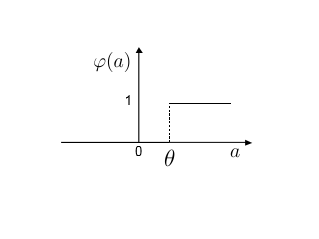
\includegraphics[width=0.6\linewidth]{IMMAGINI/asoglia1}
			\caption{ Funzione a soglia senza contributo $x_{0}$ }
			\label{fig:asoglia1}
		\end{figure}
		
		\clearpage
		A volte è opportuno che la funzione di attivazione assuma valori tra $–1$ e $+1$ ed in questo caso la funzione a soglia, che diviene la ben nota \emph{funzione segno} è ridefinita così : 
	
		\begin{equation}
			\label{eqn:sistemafunzionesegno} 
				$$ \begin{center} 
					$y=\varphi(a)=$
						$\begin{cases}
							1 \hspace{1.1cm}se\hspace{0.1cm} a>0 \\
							0 \hspace{1.1cm}se\hspace{0.1cm} a=0 \\
				    		-1 \hspace{0.8cm}se\hspace{0.1cm} a<0
						\end{cases}$
				\end{center} $$
		\end{equation}
	
		
		\subsection{Funzione lineare}
	
		Se $a=\sum\limits_{i=0}^n w_{i}x_{i}$, si avrà:
	
		\begin{equation}
		\label{eqn:sistemafunzionelineare} 
			$$ \begin{center} 
					$y=\varphi(a)=a$
			\end{center} $$
		\end{equation}

		Il grafico rispettivo
		\begin{figure}[h]
			\centering
			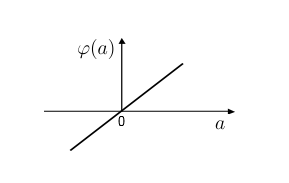
\includegraphics[width=0.6\linewidth]{IMMAGINI/lineare}
			\caption{ Funzione lineare }
			\label{fig:lineare}
		\end{figure}
	
		\clearpage
		\subsection{Funzione lineare a tratti}
	
		Un esempio di funzione di attivazione lineare a tratti è:
	
		\begin{equation}
		\label{eqn:sistemafunzionelineareatratti} 
			$$ \begin{center} 
				$y=\varphi(a)=$
					$\begin{cases}
						1 \hspace{1.86cm}se\hspace{0.1cm} a \leq -0.5 \\
						a+0.5 \hspace{0.8cm}se\hspace{0.1cm} -0.5<a<0.5\\
						0 \hspace{1.86cm}se\hspace{0.1cm} a\geq0.5 
					\end{cases}$
			\end{center} $$
		\end{equation}
	
		Che rappresentata è
		\begin{figure}[h]
			\centering
			\includegraphics[width=0.6\linewidth]{"IMMAGINI/a tratti"}
			\caption{ Funzione a tratti }
			\label{fig:atratti}
		\end{figure}

		\subsection{Funzione sigmoide}
	
		La funzione sigmoide appartenente alla famiglia di funzioni continue non lineari ed è tra le più utilizzate. \\
		\clearpage
		Tra queste funzioni riportiamo la \emph{funzione logistica} così definita:
	
		\begin{equation}
			\label{eqn:sigmoide} 
			$$ \begin{center} 
				$y=\varphi(a)=\dfrac{1}{1+e^{-a}}$
				\end{center} $$
		\end{equation}
	
		imponendo sempre $a=\sum\limits_{i=0}^n w_{i}x_{i}$.
	
		Essa assume questa forma
		\begin{figure}[h]
			\centering
			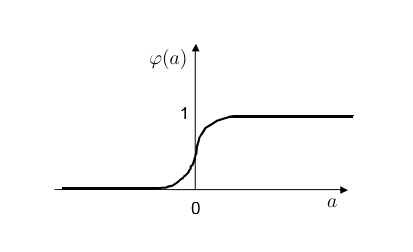
\includegraphics[width=0.6\linewidth]{IMMAGINI/sigmoide}
			\caption{ Funzione sigmoide }
			\label{fig:sigmoide}
		\end{figure}
	
		
		\section{Architettura di una rete neurale }
		
		L'architettura di una rete neurale artificiale è caratterizzata da:
		
		\begin{itemize}
			\item Numero di strati di sinapsi;
			\item Numero di neuroni presenti nell'\emph{input layer}, ovvero lo strato di ingresso;
			\item Numero di neuroni nell'\emph{output layer}, lo strato di uscita.
		\end{itemize}
	
		\begin{figure}[h]
			\centering
			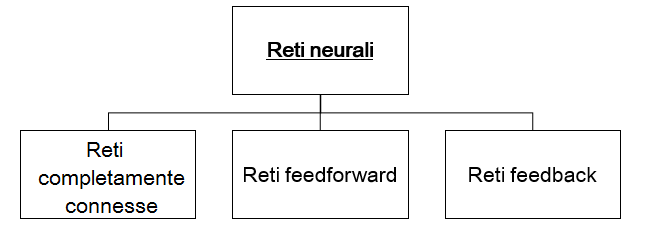
\includegraphics[width=0.7\linewidth]{IMMAGINI/diagrammareti}
			\caption{ Suddivisione delle reti neurali}
			\label{fig:diagrammareti}
		\end{figure}
		
		
		Le reti neurali si suddividono principalmente in due grandi classi: le reti \emph{feedforward} e le reti \emph{feedback} o \emph{ricorrenti}. 
		Si ha inoltre un'altra tipologia di reti che sono le \emph{reti completamente connesse}.\\
		
		\underline{\emph{Reti completamente connesse}}\\
		Nelle reti completamente connesse ogni neurone è connesso con tutti gli altri. Le connessioni tra i neuroni sono bidirezionali e possono essere rappresentate per mezzo di una matrice quadrata $W$, di dimensione pari al numero di neuroni. Un suo generico elemento $w_{i,j}$ rappresenta il peso della connessione tra il neurone $i$ ed il neurone $j$.  
		
		\begin{figure}[h]
			\centering
			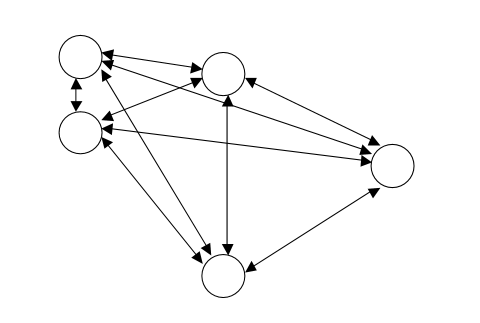
\includegraphics[width=0.7\linewidth]{IMMAGINI/completamenteconnesssa}
			\caption{ Rete completamente connessa}
			\label{fig:completamenteconnesssa}
		\end{figure}
		
		\underline{\emph{Reti feedforward a strati}}\\
		In queste reti i segnali viaggiano dallo strato di ingresso verso lo strato di uscita e pertanto vengono anche chiamate \textbf{reti feedforward}. Nelle reti stratificate non esistono connessioni tra i neuroni all'interno di uno stesso strato, nè tra neuroni di strati non limitrofi. Ogni neurone in un generico strato è connesso con tutti quelli dello strato successivo ed i neuroni dello strato di ingresso hanno come unico compito quello di trasmettere i segnali ricevuti allo strato successivo, all'interno di essi non avviene alcuna computazione.\\
		Le reti feedforward a strati si distinguono in base al numero di strati che presentano, numero che dipende dallo specifico problema che si intende risolvere.\\ 
		- \emph{Reti feedforward ad uno strato} : questa è una forma semplice di reti a strati. Il segnale nella rete si propaga in avanti senza cicli, \textbf{NON} ci sono connessioni che tornano indietro e nemmeno connessioni trasversali nel layer di output.\\
		- \emph{Reti feedforward a più strati }: le reti a più strati sono anche dette \textit{reti multilivello }, in inglese \textbf{\textit{}Multi-Layer Perceptron, MLP}. Tra l'input layer e l'output layer sono presenti uno o più strati di neuroni nascosti, si parla quindi di \textit{\textit{hidden layers}} Nelle MLP non esistono connessioni nè tra neuroni di uno stesso strato nè tra neuroni di strati non limitrofi. Ogni strato ha connessioni entranti dal precedente strato e uscenti in quello successivo, quindi la propagazione del segnale avviene in avanti in modo aciclico e senza connessioni trasversali.\\
		Tali reti vengono utilizzate per superare problemi che possono sorgere nella discriminazione dei segnali: attraverso i neuroni nascosti si ottengono delle rappresentazioni interne dei segnali di input che consentono il riconoscimento di forme più complesse, facilitando il compito della rete. 
		Nonostante tutto, però, l’aggiunta di ulteriori strati nascosti non ottimizza le abilità di discriminazione della rete; questo è possibile solo se la funzione di attivazione è non lineare (una rete multistrato a neuroni lineari è sempre riconducibile ad una rete con due soli strati).\\ 
		
		\clearpage
		\begin{figure}[h]
			\centering
			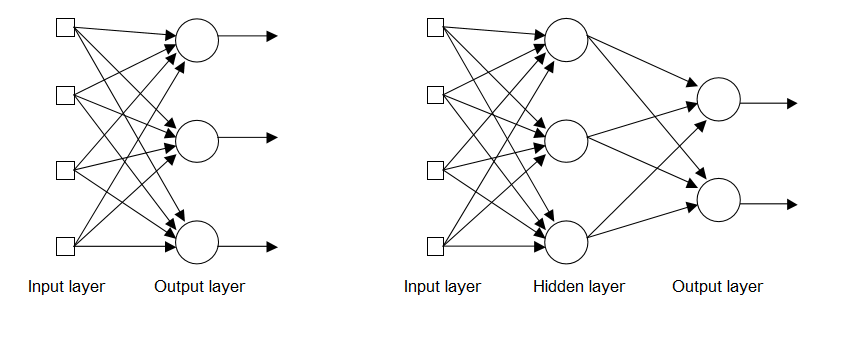
\includegraphics[width=1\linewidth]{IMMAGINI/unostrato}
			\caption{Rete ad uno strato (a sinistra), rete multilivello (a destra)}
			\label{fig:multistrato}
		\end{figure}
	
		\underline{\emph{Reti ricorrenti}}\\
		Una rete neurale ricorrente (RNN) si distingue dalle precedenti nel fatto che è ciclica. Il sistema è dinamico, le unità di output sono connesse con quelle intermedie e con quelle di input, si ha una \emph{retroazione}. Dato un determinato stimolo, la risposta della rete ricorrente non viene dettata soltanto dai caratteri strutturali della rete stessa, come si verifica nella rete feedforward, ma varia in funzione del precedente contesto in cui si è manifestato lo stimolo. L'output non è determinato solo dall'input, ma anche da una \emph{cronologia} di input che fornisce una forma di memoria a breve termine. Queste reti sono adatte per dati strutturati temporalmente ed hanno anche la possibilità di avere un’attività in assenza di una stimolazione input, poiché gli impulsi che viaggiano sulle vie ricorrenti possono essere sufficienti a mantenere il sistema in attività.
	
%FINE PRIMO CAPITOLO%

%INIZIO DEL SECONDO CAPITOLO%
	
	\chapter{L'apprendimento delle reti neurali}
	
	
	
	\section{Addestramento e generalizzazione}
		
		Per costruire una rete neurale efficiente, un passo fondamentale è individuare un \textbf{insieme di apprendimento} ed un \textbf{algoritmo di apprendimento}.\\
		Per insieme di apprendimento si intende una collezione di esempi, chiamata \textbf{(cioè un)} \textbf{training set}, dai quali la rete può attingere per raggiungere lo scopo per il quale è stata progettata; per algoritmo, invece, un procedimento che permetta di prelevare le informazioni dall'insieme di apprendimento e di fissare dei parametri che vengano poi modificati attraverso operazioni iterative interfaccianti con l'ambiente.\\
		L’apprendimento avviene sempre grazie ad un certo numero di esempi prelevati dal mondo reale ed opera in due fasi distinte: 
		
		\begin{itemize}
			\item Fase di apprendimento o addestramento nota come \textbf{learning} o \textbf{training};\\
			\item Fase di generalizzazione nota come \textbf{recall}.
		\end{itemize} 
		
		Durante la fase di learning si cerca di far imparare alla rete tutte le informazioni contenute nel training set, ottenendo un modello che verrà poi utilizzato nella fase di generalizzazione per analizzare nuovi ingressi.\\  
		L’architettura della rete neurale gioca un ruolo fondamentale per l’efficienza nella fase di apprendimento. Non bisogna però immaginare che con l'aumentare del numero di unità, cresce il potere computazionale della rete. Infatti, in tal caso, ci si troverebbe di fronte ad una situazione di \emph{overfitting}, un adattamento forzato della rete dato che risulterebbe avere un numero eccessivo di parametri rispetto al numero di esempi forniti. Questa situazione tende a far diminuire la capacità della rete di generalizzare su nuovi esempi originando una sorta di principio di indeterminazione dell'apprendimento che può essere affrontato con la limitazione del numero degli ingressi.\\ 
		Per \textbf{generalizzazione} di una rete, si intende la sua capacità di fornire le risposte appropriate a pattern di input che non sono mai stati incontrati. Essa risulta essere un punto di forza delle reti neurali e dipende dal numero di unità nascoste, dai pesi sinaptici e dal numero di training record.\\
		Una rete neurale ``generalizza bene" se la mappa input/output che essa genera è corretta per esempi di test mai presentati in fase di training (si assume che gli esempi di test siano tratti dalla stessa popolazione usata per generare il training set). In questi termini essa produce mappature input/output corrette anche se l’input è lievemente differente dagli esempi usati in fase di training; se però la rete viene addestrata con troppi esempi, si rischia che quest'ultima memorizzi il training set trovandosi nella condizione di \emph{overtraining}. \\ 
		Per avere una struttura ottimale della rete dal punto di vista della capacità di generalizzazione una guida adatta è il \textbf{Principio di Occam}, che suggerisce molto sulla complessità delle reti e sulla loro adeguatezza e che in relazione a queste ultime può essere enunciato nel seguente modo:
		
		\textit{``Date due reti che soddisfano l'insieme di apprendimento, la rete di minore complessità è quella che si comporta meglio su esempi non visti, cioè ha la migliore capacità di generalizzazione."}\\ 
		
		
	\section{Paradigmi di apprendimento}	
		Le reti neurali si ispirano al tratto caratteristico del sistema nervoso, ovvero la capacità di acquisire esperienza da esempi del mondo reale: per questo, oltre che di apprendimento, si parla di \emph{addestramento} delle reti neurali attraverso dei \textit{paradigmi di apprendimento}.\\
		I paradigmi di apprendimento si suddividono in:
		
		\begin{itemize}
			\item \emph{apprendimento \textbf{supervisionato} }
			\item \emph{apprendimento \textbf{non supervisionato}}
		\end{itemize}
	
		\underline{Apprendimento supervisionato}\\
		Tale paradigma presuppone un \emph{training set} cioè un set di esempi nel quale sono presenti coppie del tipo $(x_{k},y_{dk})$ dove la prima variabile indica il $k$-esimo ingresso e la seconda la $k$-esima uscita desiderata. Con $y_{k}$ si indica l'uscita reale e la si confronta con l'uscita desiderata: l'obiettivo è modificare i pesi affinché si minimizzi la differenza tra le due uscite. Il training set iniziale viene proposto ripetutamente finché $y_{k}\approx y_{dk}$, ovvero l'uscita reale sia il più simile possibile a quella desiderata, il tutto modificando i pesi in base alla legge di apprendimento scelta.\\
	
		\begin{figure}[h]
			\centering
			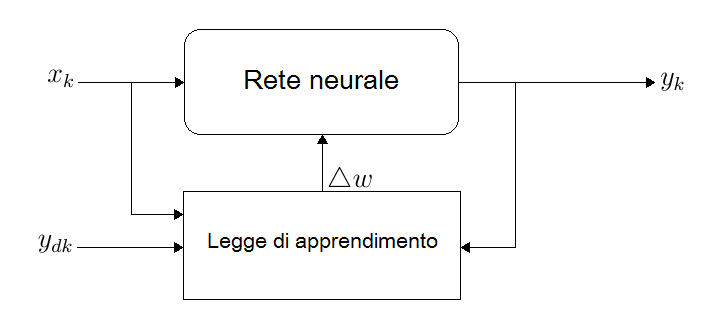
\includegraphics[width=0.7\linewidth]{IMMAGINI/supervisionato}
			\caption{ Apprendimento supervisionato }
			\label{fig:supervisionato}
		\end{figure}
		
		\clearpage
		\underline{Apprendimento non supervisionato}\\
		
		Nell'apprendimento non supervisionato la rete modifica i pesi autonomamente, si auto-organizza. Viene fornito solo il training set senza precisare le uscite.\\
	
		\begin{figure}[h]
			\centering
			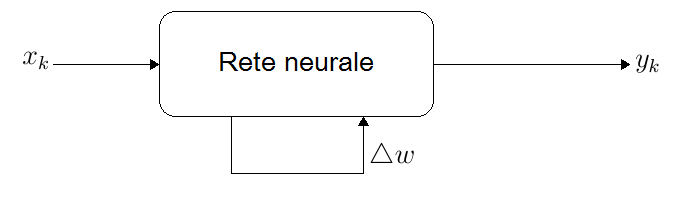
\includegraphics[width=0.7\linewidth]{IMMAGINI/nonsupervisionato}
			\caption{ Apprendimento non supervisionato}
			\label{fig:nonsupervisionato}
		\end{figure}
	
	
	\section {Processi di apprendimento}
		 
		 L’addestramento è un processo ad hoc dipendente dallo specifico problema trattato. Riportiamo alcuni processi comunemente usati .\\
		 
		 \subsection{Delta rule}
		 
		 Con regola delta, o \emph{delta rule}, si intende un apprendimento con correzione dell’errore. 
		 Siano:\\
		 $\overline{x}_{k}=[x_{1}, x_{2}, ..., x_{n}]^{T}$ il vettore $k$-esimo degli ingressi,\\ 
		 $\overline{W}_{k}=[w_{1}, w_{2}, ..., w_{n}]^{T}$ il vettore dei pesi al $k$-esimo ingresso,\\
		 e siano $y_{k}$ ed $y_{dk}$ rispettivamente l'uscita ottenuta e l'uscita desiderata.\\
		 \clearpage
		 Definiamo l'\emph{errore} come:
		
		 \begin{equation}  
			 $$ \begin{center} $\delta_{k}=y_{k}-y_{dk} $ \end{center} $$
		 \end{equation} 
	
		 Allora se consideriamo la variazione del generico vettore dei pesi $\overline{W}_{k}$ si ha che:
		 
		 \begin{equation}  
		 	$$ \begin{center} $\triangle\overline{W}_{k}=\eta\overline{x}_{k}\delta_{k}$ \end{center} $$
		 \end{equation}
		 
		 Il numero $\eta$ che compare nell'equazione (2.2) è compreso tra $0$ ed $1$, prende il nome di \textbf{learning rate} ed indica la velocità di apprendimento del neurone.\\
		 Questa regola modifica in maniera proporzionale solo i pesi delle connessioni che hanno contribuito all'errore.\\
		 L'algoritmo è il seguente:
		 
		 \begin{itemize}
		 	\item 1 - se $y_{k}=y_{dk}$ nessuna modifica dei pesi
		 	\item 2 - se $y_{k}\neq y_{dk}$ allora $\triangle\overline{W}_{k}=\eta\overline{x}_{k}\delta_{k}$.
		 \end{itemize}
		 
		 
		 \subsection{Apprendimento con correzione di errore o metodo discesa del gradiente}
		 
		 Se indichiamo con $y_{k}$ una risposta generata da un segnale di stimolo $x$ in un tempo $t$ ed indichiamo con $y_{dk}$ la risposta desiderata, avremo un \emph{segnale di}\\
		 \clearpage \emph{errore} che può essere così espresso:
		 
		 \begin{equation}
		 	$$\begin{center} $\delta= y_{dk}-y_{k}$ \end{center}$$
		 \end{equation}
		 
		 Tale segnale dà il via ad un meccanismo di controllo che va ad applicare una sequenza di modifiche ai pesi sinaptici del neurone interessato, al fine di avvicinare la risposta ottenuta a quella desiderata.\\
		 
		 \begin{figure}[h]
		 	\centering
		 	\includegraphics[width=0.7\linewidth]{"IMMAGINI/errore"}
		 	\caption{ Apprendimento con correzione }
		 	\label{fig:errore}
		 \end{figure}
		 
		
		 Questo processo di ricerca dei pesi migliori si basa sulla scelta di pesi che minimizzano una funzione errore $E(\overline{W})$, costruita al variare dei pesi stessi. \\
		 Per la scelta di tali pesi si sfruttano le informazioni fornite dal gradiente locale della funzione errore costruita.\\
		
		 \begin{figure}[h]
		 	\centering
		 	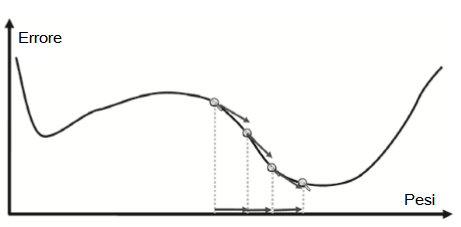
\includegraphics[width=0.7\linewidth]{IMMAGINI/gradiente}
		 	\caption{Metodo della discesa del gradiente}
		 	\label{fig:gradiente}
		 \end{figure}
		
		 Se con $\nabla_ {w}E(\overline{W})$ indichiamo il gradiente della funzione, allora:
		 
		 \begin{equation}
			 $$\begin{center} $\Delta W \varpropto \nabla_ {w}E(\overline{W}) $ \end{center}$$
		 \end{equation}
		 
		 La ricerca risulta quindi essere guidata in modo proporzionale e dato che:\\
		
		\begin{equation}
		 $$\begin{center}
		 	 $\frac{dE(\overline{w})}{d\overline{w}}=\nabla_ {w}E(\overline{w})=( \frac{\partial E(\overline{w})}{\partial w_{1}}, \frac{\partial E(\overline{w})}{\partial w_{2}}, ... ,\frac{\partial E(\overline{w})}{\partial w_{n}} )^{T}$
		 \end{center}$$
		\end{equation}
		 
	 	si avrà:
	 	
	 	\begin{equation}
	 		$$\begin{center}
	 			$\triangle\overline{W_{k}}=\eta\frac{dE(\overline{w})}{d(\overline{w})}$
	 		\end{center}$$
	 	\end{equation}
	 	
	 	Se consideriamo la $k$-esima uscita $y_{k}$ e la rispettiva uscita desiderata $y_{dk}$ ed indichiamo con $g$ la funzione di attivazione:
	 	
	 	\begin{equation}
	 		\label{eqn:coppiagradiente} 
	 			$$\begin{center} 
	 					$\begin{cases}
	 						y_{k}=g(net_{k})\\
	 						\delta_{k}=y_{k}-y_{dk} 	
	 					\end{cases}$
	 			\end{center} $$
	 	\end{equation}
	 	
	 	Si definisce l'\textbf{errore quadratico medio}:
	 	
	 	\begin{equation}
	 		$$\begin{center}
	 		$E_{k}=\frac{1}{2}(y_{k}-y_{dk})^{2}$
	 		\end{center}$$
	 	\end{equation}
	 	
		 Ma allora se consideriamo l'$i$-esimo peso del $k$-esimo input si avrà che:
		 
		 \begin{equation}
		 	$$\begin{center}
				 $\triangle{w_{i}}=\eta\frac{\partial E_{k}}{dw_{i}}$
		 	\end{center}$$
		 \end{equation}
		 
		 e sviluppando:
		 
		 \begin{equation}
		 	$$\begin{center}
		 	$\frac{\partial E_{k}}{dw_{i}}=
		 	\dfrac{\partial}{\partial w_{i}}[\frac{1}{2}(y_{k}-y_{dk})^{2}] =
		 	(y_{k}-y_{dk}) \frac{\partial (y_{k}-y_{dk})}{\partial w_{i}} =
		 	(y_{k}-y_{dk})\frac{\partial y_{k}}{\partial w_{i}}=
		 	(y_{k}-y_{dk})\frac{\partial g(net_{k})}{\partial w_{i}}=
		 	(y_{k}-y_{dk})\frac{\partial g(net_{k})}{\partial net_{k}}\frac{\partial net_{k}}{\partial w_{i}}=
		 	\delta_{k} g'(net_{k}) x_{i} $
		 \end{center}$$
		 	\end{equation}
		 	
		 	Quindi il peso $w_{i}$ sarà modificato:
		 	
		 	\begin{equation}
		 		$$\begin{center} $\triangle{w_{i}}=\eta\frac{\partial E_{k}}{dw_{i}}=\eta\delta_{k} g'(net_{k}) x_{i}$ 
		 		\end{center}$$	
		 	\end{equation}
		 
		\subsection{Apprendimento di Hebbian}
		
		Come nella delta rule, definiamo:\\
		$\overline{x}_{k}=[x_{1}, x_{2}, ..., x_{n}]^{T}$ il vettore $k$-esimo degli ingressi,\\ 
		$\overline{W}_{k}=[w_{1}, w_{2}, ..., w_{n}]^{T}$ il vettore dei pesi al $k$-esimo ingresso,\\
		e siano $y_{k}$ ed $y_{dk}$ rispettivamente l'uscita ottenuta e l'uscita desiderata.\\
		
		Nell'apprendimento di tipo hebbiano viene modificato ogni valore del peso di una connessione in questo modo:
		
		\begin{equation}  
			$$ \begin{center} $\triangle\overline{W}_{k}=\eta\overline{x}_{k}y_{dk}$ \end{center} $$
		\end{equation}
		
		con $\eta$ learning rate.\\
		I passi dell'algoritmo sono i seguenti:
		\begin{itemize}
			\item 1- se $y_{k}=y_{dk}$ nessuna modifica pesi
			\item 2- se $y_{k}>y_{dk}$ allora $\triangle\overline{W}_{k}=-\eta\overline{x}_{k}y_{dk}$
			\item 3- se  $y_{k}<y_{dk}$ allora $\triangle\overline{W}_{k}=\eta\overline{x}_{k}y_{dk}$
		\end{itemize}
		
		
		\subsection{Apprendimento competitivo}
		 
		 Tale apprendimento si basa su una vera a propria competizione tra i neuroni di uscita di una rete neurale per attivarsi in seguito ad uno stimolo. In un certo momento $t$ può attivarsi un solo neurone che viene denominato \textbf{winners-takes-all}.\\  
		 In tale processo è importare avere quindi un meccanismo che permetta ai neuroni di competere ed un valore che indichi il limite della ``forza" di ciascun neurone.\\
		 Nella forma più semplice, la rete neurale ha un solo strato di neuroni di uscita, completamente connessi ai nodi di input e che possono essere connessi tra loro.\\
		
		 \begin{figure}[h]
		 	\centering
		 	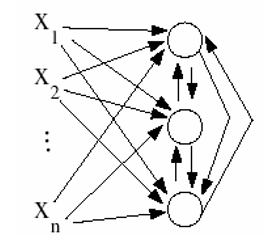
\includegraphics[width=0.4\linewidth]{IMMAGINI/competitivo}
		 	\caption{ Struttura rete con apprendimento competitivo}
		 	\label{fig:competitivo}
		 \end{figure}
		 
		 Il neurone $k$ che si attiva è quello con input netto $\nu_{k}$ più alto per un dato input $x$, con $\nu_{k}$ combinazione lineare di tutti gli input. Il suo segnale di output $y_{k}$ sarà $1$, mentre quello degli altri neuroni rimasti inattivi è $0$.
		 
		 \begin{equation}
		 \label{eqn:competitivo} 
		 	$$\begin{center} 
		 		$y_{k}=$
		 		$\begin{cases}
		 				1 \hspace{0.8cm}se\hspace{0.1cm} \nu_{k}>\nu{j} \hspace{0.6cm} \forall j,\hspace{0.2cm} j\neq k;\\
		 				0\hspace{0.8cm} altrimenti
		 			\end{cases}$
		 	\end{center} $$
		 \end{equation}
		 
		 Ora se indichiamo con $w_{k,j}$ i pesi tra il neurone $k$ e l'input $j$, supponendo che ogni neurone abbia un ammontare di peso sinaptico fisso $\sum\limits_{j} w_{kj}=1, \forall k$, il neurone che vince apprende spostando i pesi dagli input inattivi agli input attivi utilizzando tale regola:
		 
		 \begin{equation}
		 \label{eqn:competitivo} 
		 	$$\begin{center} 
		 		$\triangle w_{kj}=$
		 			$\begin{cases}
						\eta(x_{j}-w_{kj}) \hspace{0.8cm}se\hspace{0.1cm} il\hspace{0.1cm} neurone\hspace{0.1cm} k\hspace{0.1cm} vince;\\
		 				0\hspace{2.7cm} altrimenti
		 			\end{cases}$
		    \end{center} $$
		 \end{equation}
	
	
	\section{Attività di apprendimento}
		
		La scelta del paradigma di apprendimento, e quindi la metodologia di addestramento di una rete neurale, avviene in base all'attività che la rete deve svolgere, ovvero il problema che deve risolvere. Le reti neurali possono essere utilizzate come \emph{classificatori}, in grado cioè di riconoscere oggetti appartenenti a diverse categorie o possono essere responsabili dell'approssimazione di funzioni. Data una funzione nota per punti, di cui non si conosce la forma analitica, il compito della rete neurale è quello di approssimarla nel modo migliore possibile, calcolandone il valore anche in punti diversi da quelli proposti in ingresso.\\
		
		\subsection{Associazione di pattern e memoria associativa}
		
		Per memoria associativa intendiamo un criterio di memorizzazione e recupero di informazioni attraverso l'associazione. Completamente ispirata al metodo di memorizzazione del cervello umano, consente il recupero dell'informazione sulle basi di una conoscenza parziale del suo contenuto senza conoscerne la locazione di memoria.\\
		La memoria associativa si articola in due fasi:\\
		
		\begin{itemize}
		 \item Fase di memorizzazione: la rete viene addestrata per fare in modo che dei \emph{pattern}, vettori di numeri reali, vengano memorizzati ed associati;
		 \item Fase di richiamo: si richiama dalla rete un pattern memorizzato a seguito della presentazione di una versione parziale o distorta di un pattern chiave. 
		\end{itemize}
	
		Le \emph{associazioni} possono essere di due forme:\\ 
		- \underline{\emph{Autoassociazioni}}: generalmente utilizzate nell'apprendimento non supervisionato, la rete neurale memorizza un insieme di pattern che vengono ripetutamente presentati. Tra essi ne viene presentato in particolare uno che risulta essere distorto o in forma parziale. L'obiettivo è che la rete riconosca il pattern e ne richiami la versione completa/originale precedentemente memorizzata.\\
		-  \underline{\emph{Eteroassociazioni}}: ogni pattern è associato ad un altro pattern. Se $x_{k}$ è un generico pattern chiave associato al pattern memorizzato $y_{k}$, allora $x_{k}$ opera in modo tale da richiamare $y_{k}$.
		
		\subsection{Riconoscimento di pattern}
		
		Tale processo si articola in due fasi: la prima fase consiste in una sessione di addestramento in cui  alla rete vengono presentati ripetutamente un insieme di pattern specificando per ognuno la classe di appartenenza; nella seconda fase alla rete viene presentato un pattern mai mostrato precedentemente, ma appartenente ad una categoria di pattern che la rete ha memorizzato. La rete neurale sarà in grado di riconoscerne la categoria e classificare il pattern grazie ai dati precedentemente acquisiti.\\
		Il sistema è diviso in tre spazi:\\
		
		\begin{itemize}
		\item Lo \emph{spazio dei dati} costituito da tutti i pattern, un generico pattern $x$ identifica un punto dimensionale di tale spazio;
		\item Lo \emph{spazio delle caratteristiche} all'interno del quale sono presenti dei punti $y$;
		\item Lo \emph{spazio decisionale} multidimensionale suddiviso in regioni determinate dalla rete nella fase di addestramento, ognuna delle quali è associata ad una classe.
		\end{itemize}.
		
		\begin{figure}[h]
			\centering
			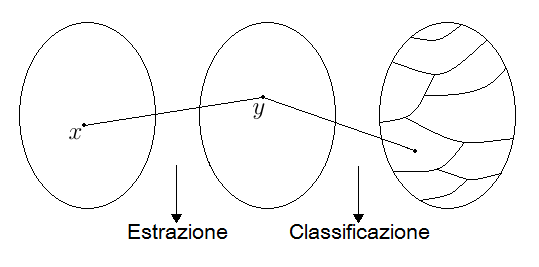
\includegraphics[width=0.7\linewidth]{IMMAGINI/classificazione}
			\caption{ Classificazione di pattern }
			\label{fig:classificazione}
		\end{figure}
		
		Il processo di riconoscimento inizia con l'estrazione delle \emph{features} ovvero le caratteristiche che un generico pattern nello spazio dei dati deve rispettare. L'\emph{estrazione} è una trasformazione che collega il pattern $x$ con un punto $y$ nello spazio delle caratteristiche. Infine un'ultima trasformazione detta \emph{classificazione} mappa dal punto $y$ in una regione dello spazio decisionale.\\
		
		\subsection{Approssimazione di funzioni}
		
		Si prenda in esame una rappresentazione non lineare input/output descritta da $y=f(x)$ dove $x$ è l'input e $y$ è l'output e si consideri un insieme di esempi ${(x_{i},y_{i} )}$ per $i=1, 2, ..., n$. L'incognita è la funzione $f$ ed il problema consiste nel creare una rete capace di generare una rappresentazione $F$ quanto più vicina alla funzione $f$. In senso euclidiano bisogna soddisfare la condizione\\
		
		\begin{center} $ ||F(x)-f(x)<\varepsilon|| \hspace{0,7cm} \forall x $ \end{center}
		
		dove $\varepsilon$ è un numero positivo piccolo, che risulterà essere sempre più piccolo con l'accrescere delle dimensioni e dei parametri liberi della rete. 
		
	
		
	\section{Un esempio di apprendimento supervisionato: il percettrone elementare}
	
		\begin{figure}[h]
			\centering
			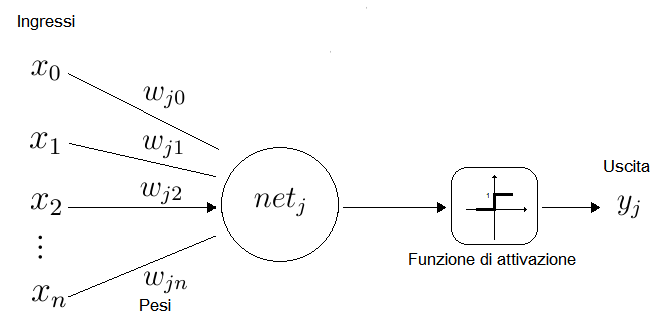
\includegraphics[width=0.7\linewidth]{IMMAGINI/perceptron}
			\caption{ Il percettrone }
			\label{fig:perceptron}
		\end{figure}	
	
		Proposto da Rosenblatt, il percettrone è la forma più semplice di rete neurale e coincide con la struttura del neurone formale. Esso è costituito da un singolo neurone in cui confluiscono più ingressi i cui pesi sinaptici sono modificabili. La funzione di attivazione è una funzione a gradino detta \emph{funzione di Heavside}:
		
		\begin{equation}
			\label{eqn:Heavside} 
				$$\begin{center} 
					$g(net_{j})=$
						$\begin{cases}
							1 \hspace{0.8cm}se\hspace{0.1cm} net_{j} \geq 0 \\
							0 \hspace{0.8cm}se\hspace{0.1cm} net_{j} < 0
						\end{cases}$
				\end{center} $$
	 	\end{equation}
		
	 	Il percettrone divide lo spazio di ingresso in due regione mediante l'iperpiano in $\Re^{n}$ di equazione: 
	 
	 	\begin{equation}  
	 		$$ \begin{center} $ w_{0}+\sum\limits_{i=1}^n w_{i}x_{i}=0 $ \end{center} $$
	 	\end{equation} 
		
		ed è quindi in grado di risolvere solo problemi \emph{linearmente separabili}.\\ 
		Supponiamo di voler classificare in due classi distinte, $C_{1}$ e $C_{2}$, oggetti rappresentati mediante punti nel piano e di sfruttare $n=2$ ingressi. Se le due classi sono linearmente separabili, l'iperpiano è una retta che funge da separatore lineare tra le due classi. Un oggetto sarà quindi classificato in base alla parte di semipiano in cui il suo punto di rappresentazione cadrà. \\
		
		\begin{figure}[h]
			\centering
			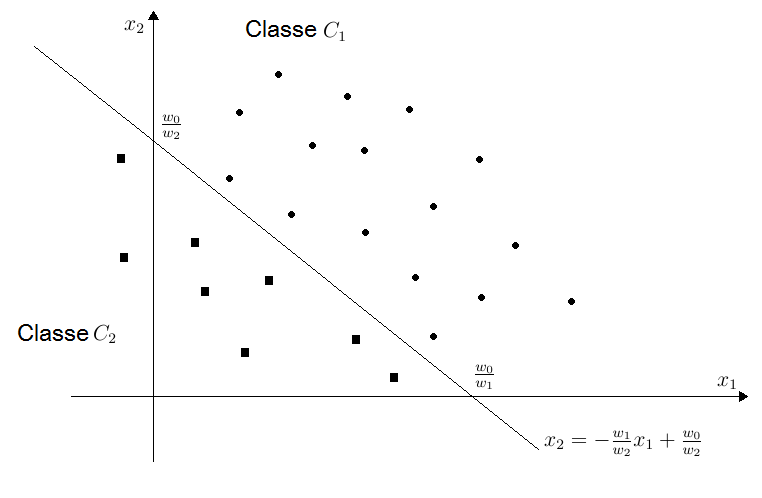
\includegraphics[width=0.7\linewidth]{IMMAGINI/rettapercettrone}
			\caption{ Separazione lineare dello spazio di ingresso di un Perceptron}
			\label{fig:rettapercettrone}
		\end{figure}
		
		Nel piano $(x_{1}, x_{2})$ degli ingressi della rete le classi $C_{1}$ e $C_{2}$ sono rappresentate da due semipiani separati dalla retta $x_{2}=-\frac{w_{1}}{w_{2}}x_{1}+\frac{w_{0}}{w_{2}}$ e possiamo classificare gli stimoli in questo modo:
		
		\begin{equation}
		 \label{eqn:semipiani} 
			$$\begin{center} 
				$\begin{cases}
						x\in C1 \hspace{0.8cm}se\hspace{0.1cm} y=1 \\
						x\in C2 \hspace{0.8cm}se\hspace{0.1cm} y=0
				\end{cases}$
			\end{center} $$
		\end{equation}
		
		
		L'apprendimento utilizzato nel perceptron è di tipo supervisionato e la learning rule attraverso i quali si modificano i singoli pesi in modo appropriato è la delta rule, definita in forma generale come:
		
		\begin{equation}  
			$$ \begin{center} $ \overline{W}_{k+1}=\overline{W}_{k}+\triangle\overline{W}_{k} $ \end{center} $$
		\end{equation} 
		
		dove $\overline{W}_{k}=[w_{1}, w_{2}, ..., w_{n}]^{T}$ è il vettore dei pesi al $k$-esimo ingresso.
		
		I passi da eseguire sono:
		
		\begin{itemize}
			\item {1 - Si inizializzano i pesi con valori casuali}
			\item {2 - Si presenta un ingresso $x_{k}$ ed il valore di uscita desiderato $y_{dk}$} 
			\item {3 - Si calcola la risposta $y_{k}$ e si aggiornano i pesi attraverso la delta rule}
			\item {4 - Si ripete il ciclo dal passo 2 finché non si ottiene una risposta soddisfacente}
		\end{itemize}
	   
	   Con riferimento alla figura 2.5, si osservi che modificando i pesi $w_{1}, w_{2}, w_{0}$ si modifica la posizione e la pendenza della retta di separazione tra le due classi. Il processo termina quando la retta separa correttamente le due classi.
	
	%FINE DEL SECONDO CAPITOLO
	
	\chapter{Ricorrenti: Reti di Hopfield}

\clearpage 
%\phantomsection 
\begin{thebibliography}{9} 
	\addcontentsline{toc}{chapter}{\refname}
	\bibitem[1]{Lazzarini} Prof.ssa Lazzarini Beatrice, (2015), \emph{Introduzione alle reti neurali.}
	\bibitem[2]{Gambosi} Prof. Gambosi Giorgio, (2010), \emph{Reti neurali, note dal corso di Machine Learning.}
	\bibitem[3]{Labonia} Prof.ssa Labonia Laura, \emph{Storia delle reti neurali artificiali.}
	\bibitem[4]{Bicego} Prof. Bicego Manuele, \emph{Riconoscimento e recupero dell’informazione per bioinformatica, reti neurali.}
	\bibitem[5]{Pioggia} Ing. Pioggia Giovanni, (2009), \emph{Modelli di sistemi fisiologici.}
 \end{thebibliography}
	
\end{document}